\documentclass[10pt,a4paper, dvipsnames]{beamer}
\usepackage[utf8]{inputenc}
\usepackage[english]{babel}
\usepackage{amsmath}
\usepackage{amsfonts}
\usepackage{amssymb}
\usepackage{graphicx}
\title{Beamer, c'est bien.}
\author{Formation \LaTeX SISEO}
\date{}

%\usetheme{Berkeley}
\usetheme{Antibes}
%\useoutertheme{split}
%\usecolortheme{structure}
%\useinnertheme[shadow=true]{rounded}
\usecolortheme[named=SeaGreen]{structure}
\setbeamercovered{transparent}
\begin{document}

\section{Introduction}
\begin{frame}
\titlepage
\end{frame}

\section{Simple slides}

\begin{frame}{A slide}

\begin{block}{A block}
Inside the block !
\end{block}

\begin{alertblock}{An alertblock}
Some text 
\end{alertblock}
\end{frame}

\section{Richer frames}
\begin{frame}{A richer frame}
  \begin{block}{A block with itemize}
    \begin{itemize}
      \item Something,
       \item Else.
    \end{itemize}
  \end{block}
\end{frame}

\section{Columns}
  \begin{frame}{A block in a column}
     \begin{columns}[c]
     \column{.5\textwidth}
     \begin{block}{A block with itemize}
       \begin{itemize}
         \item Something,
         \item Else.
       \end{itemize}
     \end{block}
     \column{.5\textwidth}
     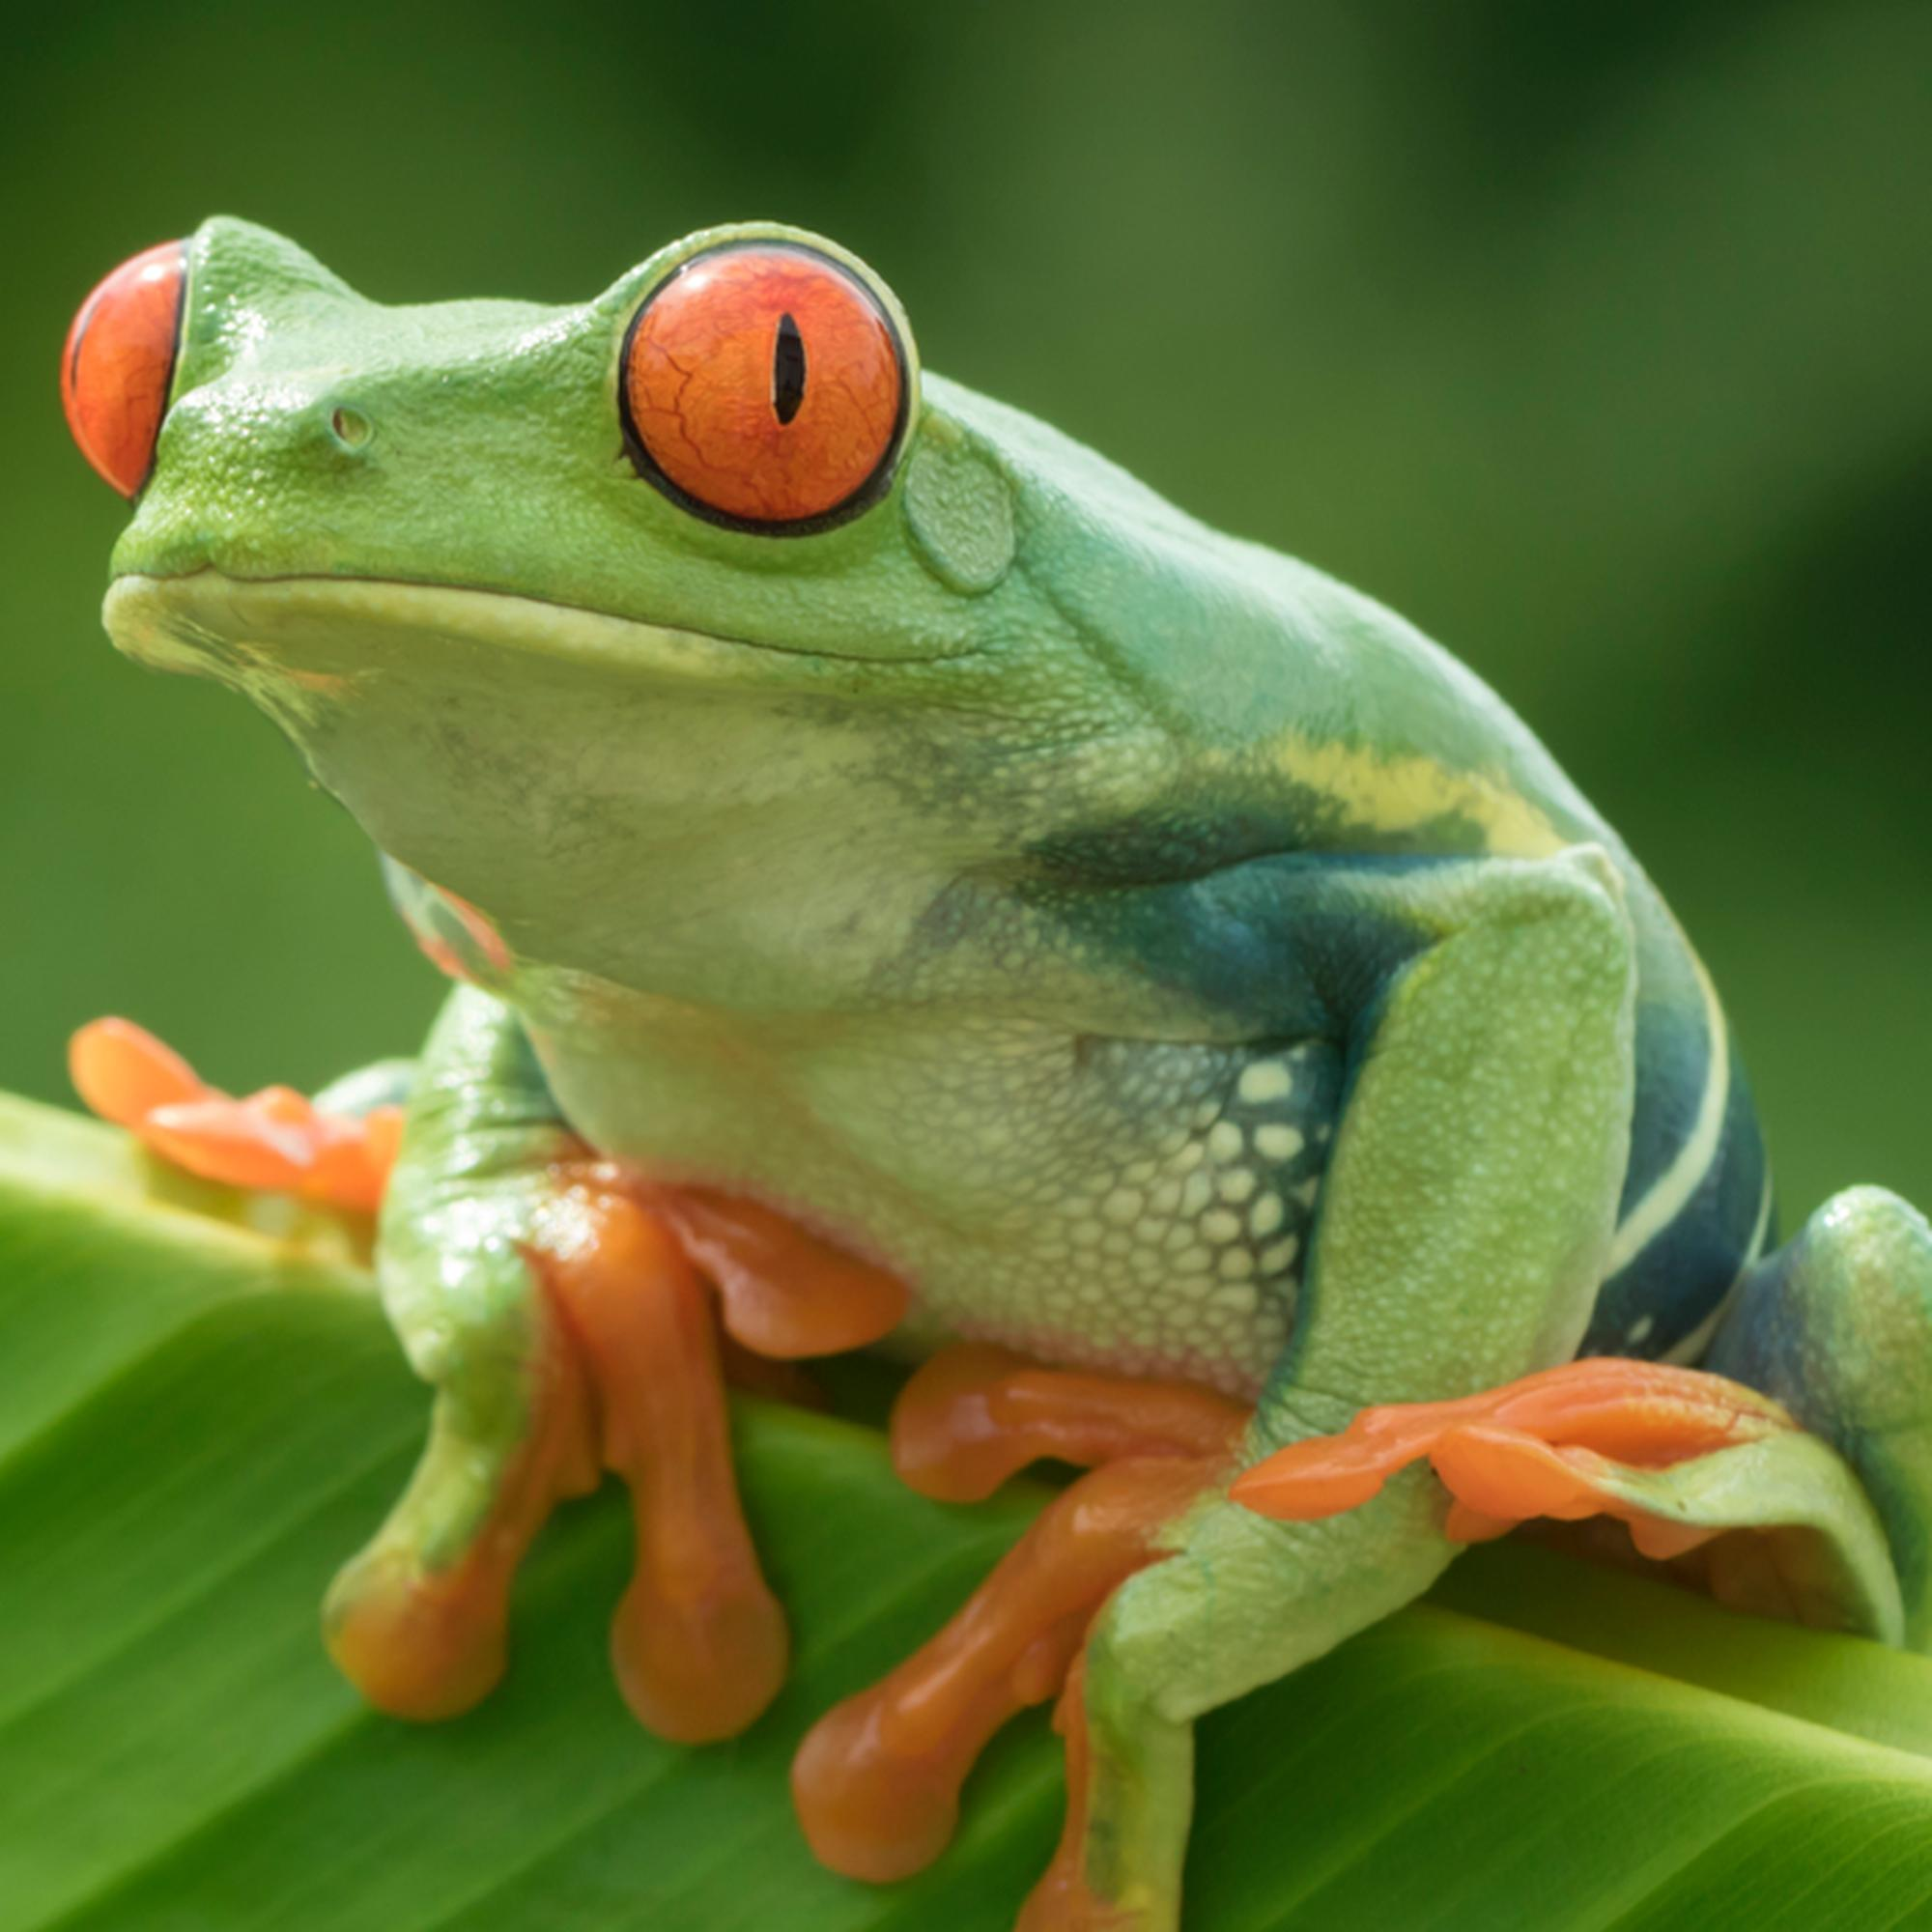
\includegraphics[width=\columnwidth]{images/frog.jpeg}
     \end{columns}
\end{frame}

\section{Overlays}


  \begin{frame}{More about frogs}
  \transsplitverticalout
     \begin{columns}[c]
     \column{.5\textwidth}
     \begin{block}{Frogs are}
       \begin{itemize}
         \item Green,
         \item<2-3> Small.
         \item<2> Stupid ?
         \item<4> Hidden ?
       \end{itemize}
     \end{block}
     \column{.5\textwidth}
     \only<1-3>{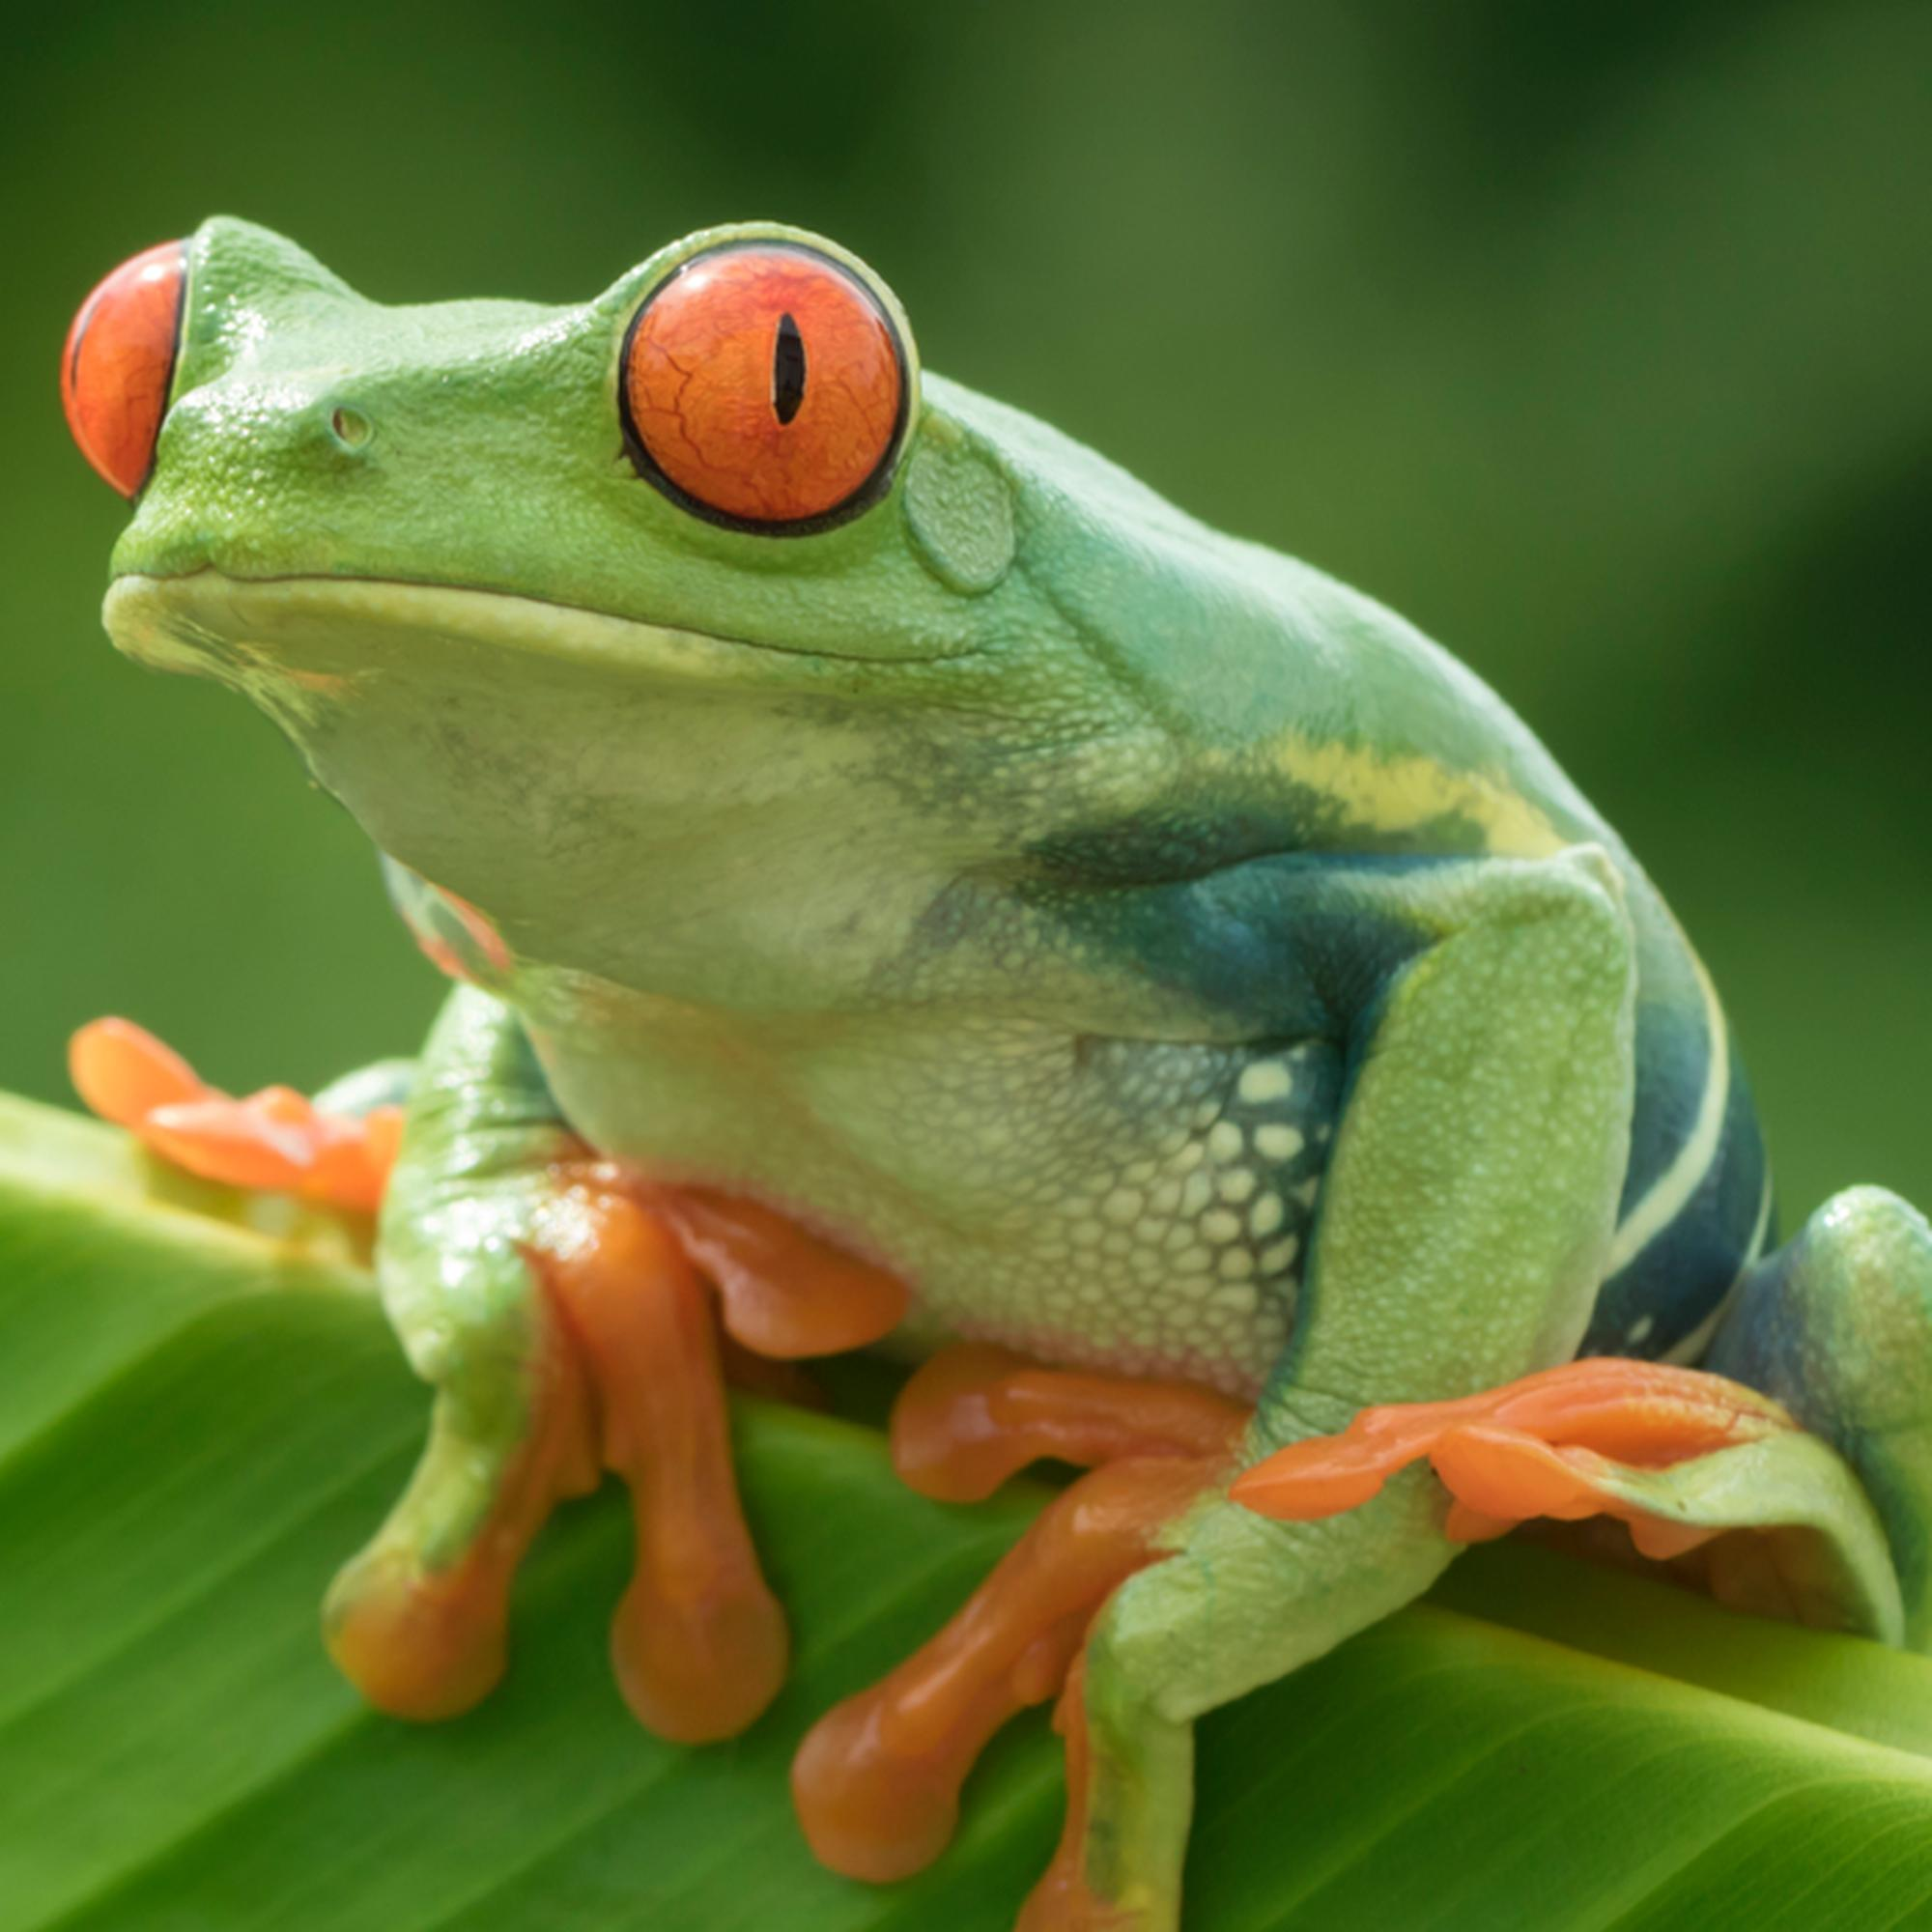
\includegraphics[width=\columnwidth]{images/frog.jpeg}}
     \end{columns}
\end{frame}

\end{document}